% Author: Dominik Harmim <harmim6@gmail.com>

%-------------------------------------------------------------------------------
%-------------------------------------------------------------------------------
%-------------------------------------------------------------------------------
%-------------------------------------------------------------------------------

\section{Introduction}

Bugs are an integral part of computer programs ever since the inception of the
programming discipline. Unfortunately, they are often hidden in unexpected
places, and they can lead to unexpected behaviour, which may cause significant
damage. Nowadays, developers have many possibilities of catching bugs in the
early development process. \emph{Dynamic analysers} or tools for \emph{automated
testing} are often used, and they are satisfactory in many cases. Nevertheless,
they can still leave too many bugs undetected, because they can analyse
only particular program flows dependent on the input data. An alternative
solution is \emph{static analysis} that has its shortcomings as well, such
as the \emph{scalability} on large codebases or a~considerably high rate of
incorrectly reported errors (so-called \emph{false positives} or \emph{false
alarms}).

Recently, Facebook introduced \emph{Facebook Infer}: a~tool for
creating \emph{highly scalable}, \emph{compositional}, \emph{incremental},
and \emph{interprocedural} static analysers. Facebook Infer has grown
considerably, but it is still under active development by many teams across
the globe. It is employed every day not only in Facebook itself, but also
in other companies, such as Spotify, Uber, Mozilla, or Amazon. Currently,
Facebook Infer provides several analysers that check for various types
of bugs, such as buffer overflows, data races and some forms of deadlocks
and starvation, null-dereferencing, or memory leaks. However, most importantly,
Facebook Infer is a~framework for building new analysers quickly and easily.
Unfortunately, the current version of Facebook Infer still lacks better
support for \emph{concurrency} bugs. While it provides a~reasonably advanced
\emph{data race} analyser, it is limited to Java and C++ programs only and
fails for C~programs, which use a~\emph{lower-level lock manipulation}.

In \emph{concurrent programs}, there are often \emph{atomicity requirements}
for execution of specific sequences of instructions. Violating these
requirements may cause many kinds of problems, such as unexpected behaviour,
exceptions, segmentation faults, or other failures. \emph{Atomicity violations}
are usually not verified by compilers, unlike syntactic or some sorts of
semantic rules. Moreover, atomicity requirements, in most cases, are not
even documented at all. So in the end, programmers themselves must abide by
these requirements and usually lack any tool support. Furthermore, in general,
it is difficult to avoid errors in \emph{atomicity-dependent programs},
especially in large projects, and even more laborious and time-consuming is
finding and fixing them.

In the thesis~\cite{harmimBP}, there was proposed
\emph{Atomer}\,--\,a~\emph{static analyser} for finding some forms of
atomicity violations implemented as a~module of Facebook Infer. In particular,
the stress is put on the \emph{atomic execution of sequences of function
calls}, which is often required, e.g., when using specific library calls.
The idea of checking atomicity of certain sequences of function calls is
inspired by the work of \emph{contracts for
concurrency}~\cite{contracts2017}. In the terminology of~\cite{contracts2017},
atomicity of specific sequences of calls is the most straightforward (yet
very useful in practice) kind of contracts for concurrency. The implementation
mainly targets C/C++ programs that use \emph{PThread} locks. Within this
project practice, Atomer was improved, extended, and other experiments were
performed. In particular, two new features were introduced:
\begin{enumerate*}[label={(\roman*)}]
    \item
        support for \emph{C++} and \emph{Java} locks,

    \item
        and a~way to distinguish \emph{multiple locks used}.
\end{enumerate*}
Moreover, working with \emph{sequences of function calls} was approximated
by working with \emph{sets of function calls} to make the solution more
\emph{scalable}.

The development of Atomer has been discussed with developers of Facebook
Infer, and it is a~part of the H2020 ECSEL project Aquas. Parts of this
report are taken from the thesis~\cite{harmimBP} and the
paper~\cite{excel2019FBInfer} written in collaboration with Vladimír Marcin
and Ondřej Pavela.

The rest of the report is organised as follows. In Section~\ref{sec:fbinfer},
there is described the Facebook Infer framework. Atomer is described in
Section~\ref{sec:atomer}, together with all the extensions and improvements
implemented within this project practice. Subsequently,
Section~\ref{sec:exp} discusses the experimental evaluation of the new
features and other experiments that were performed in this project.
Finally, Section~\ref{sec:conc} concludes the report.

%-------------------------------------------------------------------------------
%-------------------------------------------------------------------------------
%-------------------------------------------------------------------------------
%-------------------------------------------------------------------------------

\section{Facebook Infer}
\label{sec:fbinfer}

This section describes the principles and features of \emph{Facebook Infer}.
The description is based on information provided at the Facebook Infer's
website\footnote{\textbf{Facebook Infer's}
website\,--\,\url{https://fbinfer.com}.} and
in~\cite{projectPracticeMarcin2018}. Parts of this section are taken
from~\cite{harmimBP, excel2019FBInfer}.

Facebook Infer is an \emph{open-source}\footnote{\textbf{Open-source repository
of Facebook Infer} on GitHub\,--\,\url{https://github.com/facebook/infer}.}
\emph{static analysis framework}\footnote{A~brief explanation of \textbf{static
analysis} itself can be found in~\cite{harmimBP}\,--\,Section~2.1. In more
detail, it is then explained in~\cite{staticAnalysisMoller,
favStaticAnalysis}.}, which can discover various kinds of software bugs of
a~given program, with the stress put on \emph{scalability}. A~more detailed
explanation of the architecture of Facebook Infer is shown in
Section~\ref{sec:fbinferArch}. Facebook Infer is implemented in
\emph{OCaml}\footnote{\textbf{OCaml's}
website\,--\,\url{https://ocaml.org}.}\,--\,a~\emph{functional} programming
language, also supporting \emph{imperative} and \emph{object-oriented}
paradigms. Further details about OCaml can be found in~\cite{realWorldOCaml}.
Facebook Infer was originally a~standalone tool focused on \emph{sound
verification} of the absence of \emph{memory safety violations}, which was
first published in the well-known paper~\cite{inferBiabduction}.

Facebook Infer can analyse programs written in several languages. In
particular, it supports languages C, C++, Java, and Objective-C. Moreover, it
is possible to extend Facebook Infer's \emph{frontend} for supporting other
languages. Currently, Facebook Infer contains many analyses focusing on various
kinds of bugs, e.g., \emph{Inferbo} (buffer overruns)~\cite{inferboOnline};
\emph{RacerD} (data races)~\cite{racerD, racerDOnline,
staticRaceDetectorTruePositive}; and other analyses that check for buffer
overflows, some forms of deadlocks and starvation, null-dereferencing, memory
leaks, resource leaks, etc.

\subsection{Abstract Interpretation in Facebook Infer}

Facebook Infer is a~general framework for static analysis of programs, and it
is based on \emph{abstract interpretation}\footnote{\textbf{Abstract
interpretation} is explained and formally
defined in~\cite{harmimBP}\,--\,Section~2.1.1. Additional description can be
found in~\cite{AIBasedFormalMethodsCousot, AILatticeModelCousot,
AIInNutshellCousot, AICousotWeb, favAI, projectPracticeMarcin2018,
wideningNarrowingCousot, programAnalysisNielson, staticAnalysisMoller,
favLatticesAndFixpoints}.}. Despite the original approach taken
from~\cite{inferBiabduction}, Facebook Infer aims to find bugs rather than
\emph{formal verification}. It can be used to quickly develop new sorts of
\emph{compositional} and \emph{incremental} analysers (\emph{intraprocedural}
or \emph{interprocedural}~\cite{programAnalysisNielson}) based on the concept
of function \emph{summaries}. In general, a~\emph{summary} is a~representation
of \emph{preconditions} and \emph{postconditions} of a~function. However, in
practice, a~summary is a~custom data structure that may be used for storing
any information resulting from the analysis of particular functions. Facebook
Infer generally does not compute the summaries in the course of the analysis
along the \emph{Control Flow Graph}
(\textbf{CFG}~\cite{controlFlowAnalysisAllen}) as it is done in classical
analyses based on the concepts from~\cite{dataflowAnalysisGraphReachability,
dataflowAnalysisApproaches}. Instead, Facebook Infer performs the analysis of
a~program \emph{function-by-function along the call tree}, starting from its
leafs (demonstrated in Example~\ref{ex:fbinferAnalysis}). Therefore, a~function
is analysed, and a~summary is computed without knowledge of the call context.
Then, the summary of a~function is used at all of its call sites. Since
summaries do not differ for different contexts, the analysis becomes more
scalable, but it can lead to a~loss of accuracy.

In order to create a~new intraprocedural analyser in Facebook Infer,
it is needed to define the following (the listed items are described in more
detail in~\cite{harmimBP}\,--\,Section~2.1.1):
\begin{enumerate}
    \item
        The \emph{abstract domain}~$ Q $, i.e., a~type of an \emph{abstract
        state}.

    \item
        Operator~$ \sqsubseteq $, i.e., an \emph{ordering} of abstract states.

    \item
        The \emph{join} operator~$ \circ $, i.e., the way of joining two
        abstract states.

    \item
        The \emph{widening} operator~$ \triangledown $, i.e., the way how to
        enforce termination of the abstract interpretation of an iteration.

    \item
        \emph{Transfer functions}~$ \tau $, i.e., a~transformer that takes an
        abstract state as an input and produces an abstract state as an output.
\end{enumerate}
Further, in order to create an interprocedural analyser, it is required to
define additionally:
\begin{enumerate}
    \item
        The type of function summaries.

    \item
        The logic for using summaries in transfer functions, and the logic for
        transforming an intraprocedural abstract state to a~summary.
\end{enumerate}

An important feature of Facebook Infer improving its scalability is
\emph{incrementality} of the analysis. It allows one to analyse separate code
changes only, instead of analysing the whole codebase. It is more suitable for
extensive and variable projects, where ordinary analysis is not feasible. The
incrementality is based on \emph{re-using summaries} of functions for which
there is no change in them neither in the functions transitively invoked from
them.

\subsection{\sloppy%
    Architecture of the Abstract Interpretation Framework in Facebook Infer%
}
\label{sec:fbinferArch}

The architecture of the abstract interpretation framework of Facebook Infer
(\textbf{Infer.AI}) may be split into three major parts, as demonstrated in
Figure~\ref{fig:inferArch}: a~\emph{frontend}, an \emph{analysis scheduler}
(and a~\emph{results database}), and a~set of \emph{analyser plugins}.

\begin{figure}[hbt]
    \centering
    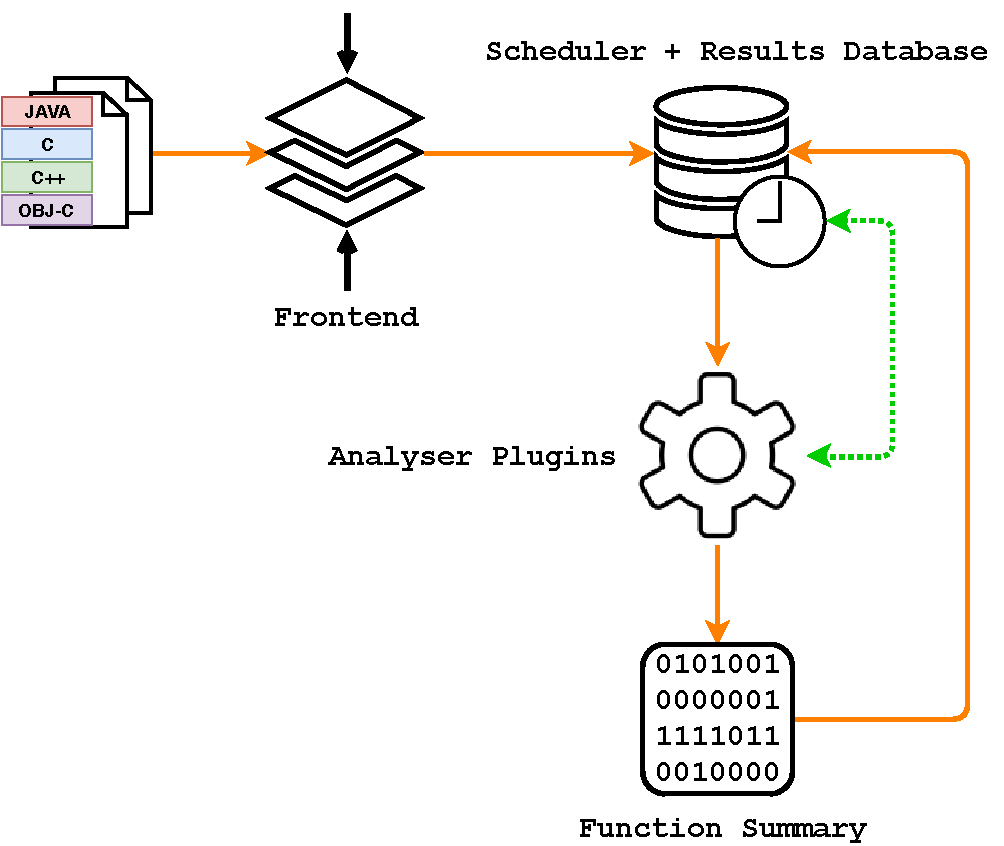
\includegraphics[width=.9 \linewidth]{infer-architecture.pdf}
    \caption{%
        The architecture of Facebook Infer's abstract interpretation
        framework~\cite{harmimBP, projectPracticeMarcin2018}
    }
    \label{fig:inferArch}
\end{figure}

The frontend compiles input programs into the \emph{Smallfoot Intermediate
Language} (SIL) and represents them as a~CFG. There is a~separate CFG
representation for each analysed function. Nodes of this CFG are formed as
instructions of SIL. The SIL language consists of the following underlying
instructions:
\begin{itemize}
    \item
        \texttt{LOAD}: reading into a~temporary variable.

    \item
        \texttt{STORE}: writing to a~program variable, a~field of
        a~structure, or an array.

    \item
        \texttt{PRUNE~e}~(often called \texttt{ASSUME}): evaluation of
        a~condition~\texttt{e}.

    \item
        \texttt{CALL}: a~function call.
\end{itemize}
The frontend allows one to propose analyses that are \emph{language-independent}
(to a~certain extent) because it supports input programs to be written in
multiple languages.

The next part of the architecture is the scheduler, which defines the order of
the analysis of single functions according to the appropriate \emph{call
graph}\footnote{\textbf{A~call graph} is a~\emph{directed graph} describing
call dependencies among functions.}. The scheduler also checks if it is possible
to analyse some functions simultaneously, which allows Facebook Infer to run
the analysis in parallel.

\begin{example}
    \label{ex:fbinferAnalysis}
    For demonstrating the order of the analysis in Facebook Infer and its
    incrementality, assume a~call graph given in
    Figure~\ref{fig:inferCallGraph}. At first, leaf functions \texttt{F5} and
    \texttt{F6} are analysed. Further, the analysis goes on towards the root of
    the call graph\,--\,\texttt{F\textsubscript{MAIN}}, while taking into
    consideration the dependencies denoted by the edges. This order ensures
    that a~summary is available once a~nested function call is abstractly
    interpreted within the analysis. When there is a~subsequent code change,
    only directly changed functions and all the functions up the call path are
    re-analysed. For instance, if there is a~change of source code of function
    \texttt{F4}, Facebook Infer triggers re-analysis of functions \texttt{F4},
    \texttt{F2}, and \texttt{F\textsubscript{MAIN}} only.
\end{example}

\begin{figure}[hbt]
    \centering
    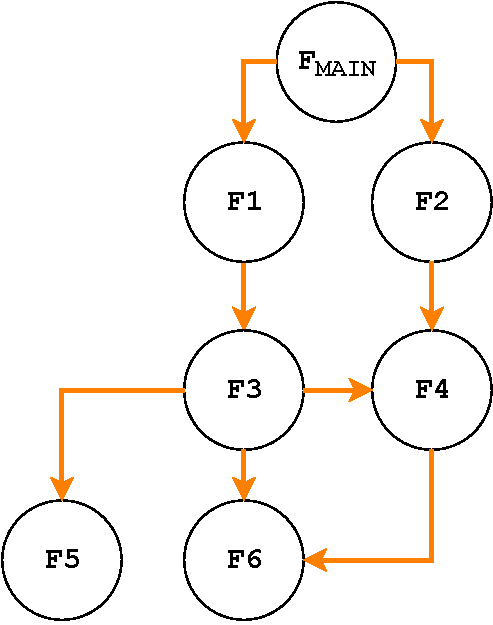
\includegraphics[width=.6 \linewidth]{infer-call-graph.pdf}
    \caption{%
        A~call graph for an illustration of Facebook Infer's analysis
        process~\cite{harmimBP, excel2019FBInfer, projectPracticeMarcin2018}%
    }
    \label{fig:inferCallGraph}
\end{figure}

The last part of the architecture consists of a~set of analyser plugins. Each
plugin performs some analysis by interpreting SIL instructions. The result
of the analysis of each function (function summary) is stored to the results
database. The interpretation of SIL instructions (\emph{commands}) is done using
an \emph{abstract interpreter} (also called a~\emph{control interpreter}) and
\emph{transfer functions} (also called a~\emph{command interpreter}). The
transfer functions take a~previously generated \emph{abstract state} of an
analysed function as an input, and by applying the interpreting command,
produce a~new abstract state. The abstract interpreter interprets the command
in an \emph{abstract domain} according to the CFG. This workflow is shown in
a~simplified form in Figure~\ref{fig:inferAnalysis}.

\begin{figure}[hbt]
    \centering
    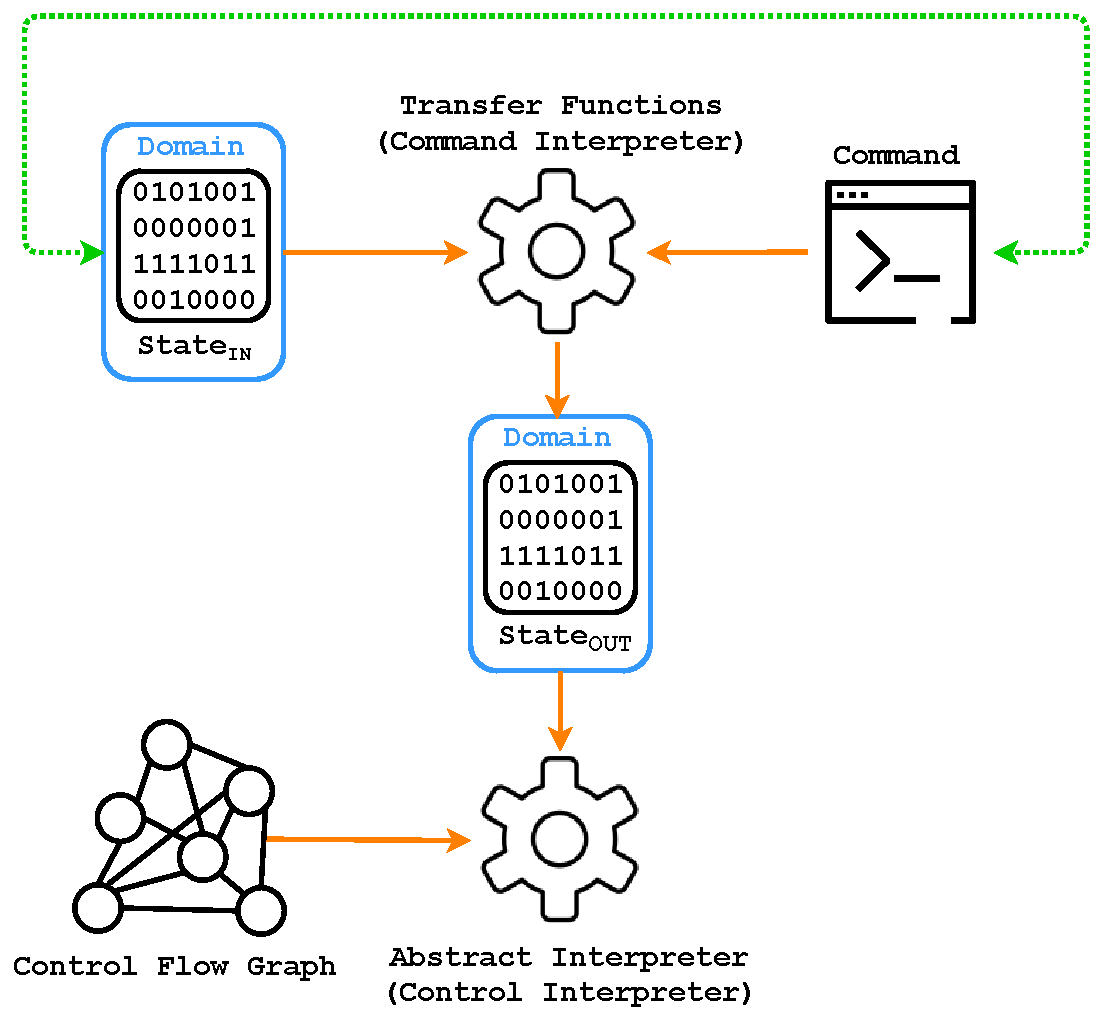
\includegraphics[width=.9 \linewidth]{infer-analysis.pdf}
    \caption{%
        Facebook Infer's abstract interpretation
        process~\cite{harmimBP, projectPracticeMarcin2018}%
    }
    \label{fig:inferAnalysis}
\end{figure}

%-------------------------------------------------------------------------------
%-------------------------------------------------------------------------------
%-------------------------------------------------------------------------------
%-------------------------------------------------------------------------------

\section{Atomicity Violations Detector}
\label{sec:atomer}

In the thesis~\cite{harmimBP} and the paper~\cite{excel2019FBInfer}, there
was proposed\ \,\emph{Atomer}\,--\,a~\emph{static analyser} for finding some
forms of \emph{atomicity violations} implemented as a~module of \emph{Facebook
Infer}. The proposed solution is slightly inspired by ideas from~\cite{contract,
contracts2017, contracts2015, muzikovskaBP, excel2018Muzikovska}.

As demonstrated in Figure~\ref{fig:atomerProposal}, the proposed analysis is
divided into two parts (\emph{phases of the analysis}):
\begin{enumerate}[label={\textbf{Phase~\arabic*}:}, leftmargin=5em]
    \item
        Detection of (likely) \emph{atomic sequences}.

    \item
        Detection of \emph{atomicity violations} (violations of the atomic
        sequences).
\end{enumerate}
The design and implementation are in detail described
in~\cite{harmimBP}\,--\,Chapters~3 and~4.

\begin{figure}[hbt]
    \centering
    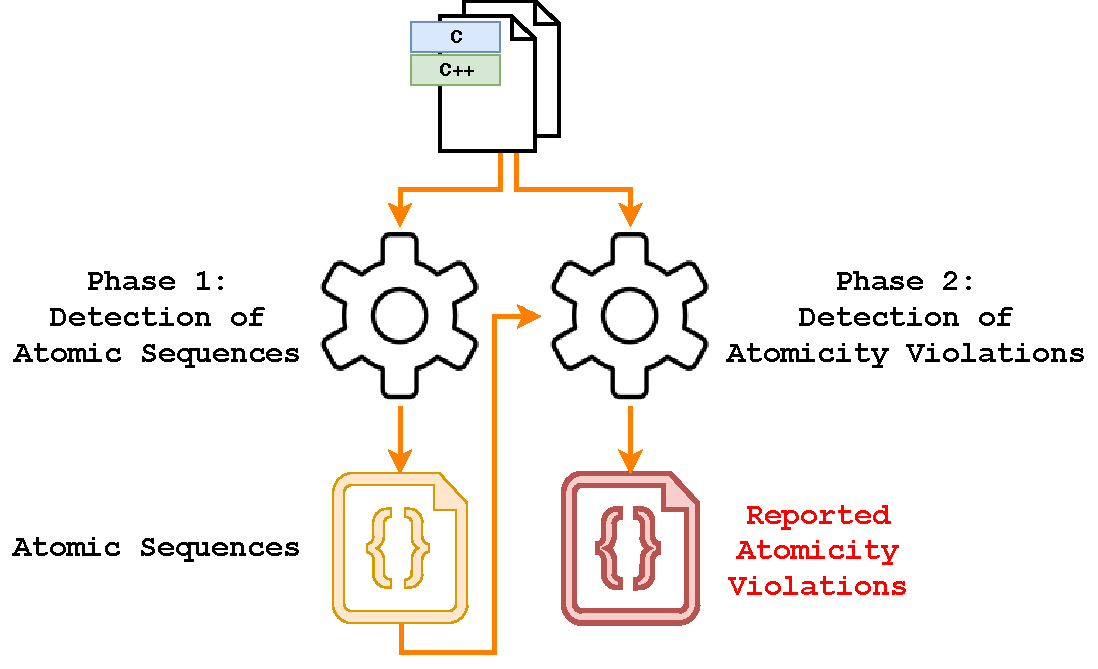
\includegraphics[width=.9 \linewidth]{analyser-proposal.pdf}
    \caption{Phases of the proposed analyser}
    \label{fig:atomerProposal}
\end{figure}

\subsection{\sloppy%
    Approximation with Sets of Function Calls%
}

In this work, the approach of~\cite{harmimBP} that worked with \emph{sequences
of function calls} was approximated by working with \emph{sets of function
calls} to make the solution more \emph{scalable}. In particular, the solution
is more scalable because the order of stored function calls is not relevant
while working with sets. Thus, less memory is required because the same sets
of function calls are not stored multiple times. The analysis is also faster
since there are stored fewer function calls to work with. On the other hand,
the analysis is less accurate because the new approach causes some loss of
information. The analysis after the approximation is illustrated in
Figure~\ref{fig:atomerProposalSets}.

\begin{figure}[hbt]
    \centering
    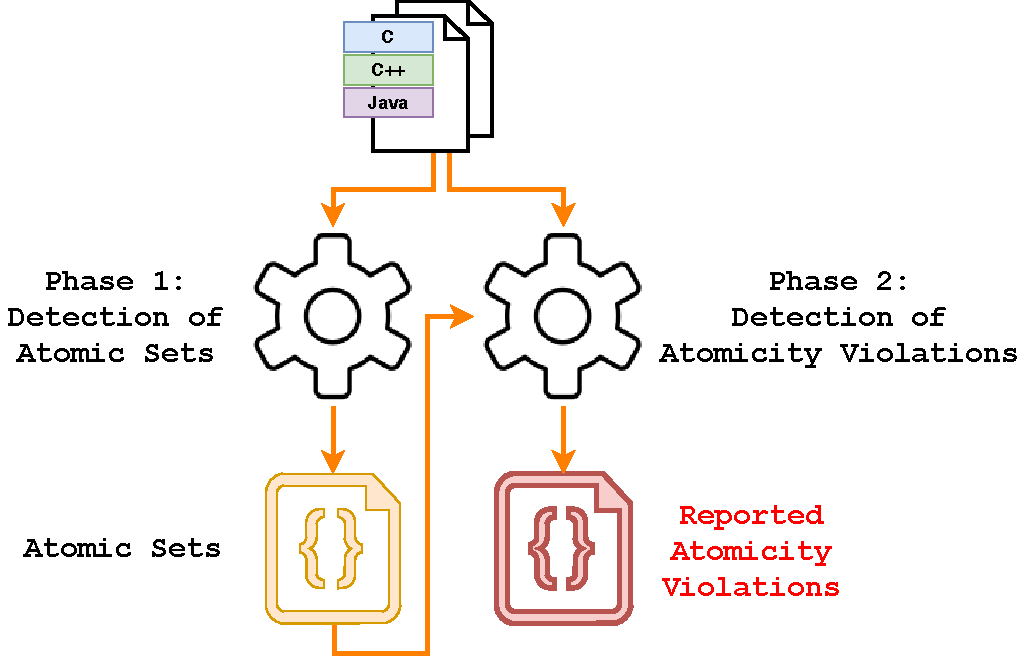
\includegraphics[width=.9 \linewidth]{analyser-proposal-sets.pdf}
    \caption{Phases of the analyser approximated with sets of function calls}
    \label{fig:atomerProposalSets}
\end{figure}

\begin{example}
    For demonstrating the approximation of the analysis with sets of
    function calls, assume functions from Listing~\ref{list:approx}.
    Before the approximation, when the analysis was working with sequences
    of function calls, \textbf{Phase~1} of the analysis produced the
    following \emph{summary} while analysing function~\texttt{f}:
    (\textcolor{red}{(\texttt{a}, \texttt{b}, \texttt{c})}, \textcolor{blue}{%
    (\texttt{x}, \texttt{a}, \texttt{b}, \texttt{c})}), and the following
    summary while analysing function~\texttt{g}:
    (\textcolor{red}{(\texttt{c}, \texttt{b}, \texttt{a})}, \textcolor{blue}{%
    (\texttt{x}, \texttt{c}, \texttt{b}, \texttt{a})}), where
    \textcolor{red}{the first component is a~sequence of atomic calls}
    and \textcolor{blue}{the second component is a~sequence of all calls}.
    Whereas, after the approximation, the produced summary for both
    functions is the same because \textcolor{red}{the first component is
    a~set of atomic calls} and \textcolor{blue}{the second component is
    a~set of all calls}: (\textcolor{red}{\{\texttt{a}, \texttt{b},
    \texttt{c}\}}, \textcolor{blue}{\{\texttt{a}, \texttt{b}, \texttt{c},
    \texttt{x}\}}).
\end{example}

\begin{lstlisting}[%
    style=c++, label={list:approx}, float=hbt, caption={%
    A~code snippet used for illustration of the approximation
    of the analysis with sets of function calls}%
]
void f(void)
{
    x();

    <@\textcolor{red}{pthread\_mutex\_lock}@>(&L);
    a(); b(); c();
    <@\textcolor{red}{pthread\_mutex\_unlock}@>(&L);
}

void g(void)
{
    x();

    <@\textcolor{red}{pthread\_mutex\_lock}@>(&L);
    c(); b(); a();
    <@\textcolor{red}{pthread\_mutex\_unlock}@>(&L);
}
\end{lstlisting}

\begin{example}
    In \textbf{Phase~2} of the analysis, if the result of the first phase
    had been the following set of sequences of functions called atomically
    \{(\texttt{a}, \texttt{b}, \texttt{c})\}, the analysis would have looked
    for the following pairs of functions that are not called atomically:
    (\texttt{a}, \texttt{b}), (\texttt{b}, \texttt{c}). Since the result
    of the first phase was changed to the following set of sets of
    functions called atomically \{\{\texttt{a}, \texttt{b}, \texttt{c}\}\},
    the analysis now looks for the following pairs of functions that are
    not called atomically: (\texttt{a}, \texttt{b}), (\texttt{b},
    \texttt{a}), (\texttt{b}, \texttt{c}), (\texttt{c}, \texttt{b}),
    (\texttt{a}, \texttt{c}), (\texttt{c}, \texttt{a}). I.e., it looks
    for all the possible pairs from a~given set.
\end{example}

\subsection{Distinguishment of Multiple Locks Used}

In the original version of Atomer designed in~\cite{harmimBP}, different
locks were not distinguished at all. Only calls of locks/unlocks were
identified, and parameters of these calls (\emph{lock objects}) were not
considered. So, if there had been several lock objects used, the analysis
would not have worked correctly. Therefore, lock objects are now
taken into consideration. They are distinguishing using Facebook Infer's
built-in mechanism called \emph{access paths}\footnote{Facebook Infer uses
\textbf{syntactic access paths} for naming heap locations via the paths used
to access them.~\cite{racerD}}. During the analysis (both phases), each
\emph{atomic section} is identified by an access path of a~lock that
guards that section.

\begin{example}
    Consider functions~\texttt{x} and~\texttt{y} from
    Listing~\ref{list:multipleLocks}. There are two lock objects
    \texttt{L1} and \texttt{L2} that are used simultaneously.
    After the extension of the distinguishment of multiple locks used, the
    analysis works as follows. In function~\texttt{x}, the analyser
    recognises that lock~\texttt{L1} guards a~set of atomic calls
    \{\texttt{a}, \texttt{b}, \texttt{c}\}, and lock~\texttt{L2} guards
    \{\texttt{b}\}. Further, in function~\texttt{y}, lock~\texttt{L1} guards
    \{\texttt{a}, \texttt{b}\}, and lock~\texttt{L2} guards \{\texttt{b},
    \texttt{c}\}.
\end{example}

\begin{lstlisting}[%
    style=c++, label={list:multipleLocks}, float=hbt, caption={%
    A~code snippet used for illustration of distinguishing
    multiple locks used}%
]
void x(void)
{
    <@\textcolor{red}{pthread\_mutex\_lock}@>(&<@\textcolor{red}{L1}@>);
    a();
    <@\textcolor{cyan}{pthread\_mutex\_lock}@>(&<@\textcolor{cyan}{L2}@>);
    b();
    <@\textcolor{cyan}{pthread\_mutex\_unlock}@>(&<@\textcolor{cyan}{L2}@>);
    c();
    <@\textcolor{red}{pthread\_mutex\_unlock}@>(&<@\textcolor{red}{L1}@>);
}

void y(void)
{
    <@\textcolor{red}{pthread\_mutex\_lock}@>(&<@\textcolor{red}{L1}@>);
    a();
    <@\textcolor{cyan}{pthread\_mutex\_lock}@>(&<@\textcolor{cyan}{L2}@>);
    b();
    <@\textcolor{red}{pthread\_mutex\_unlock}@>(&<@\textcolor{red}{L1}@>);
    c();
    <@\textcolor{cyan}{pthread\_mutex\_unlock}@>(&<@\textcolor{cyan}{L2}@>);
}
\end{lstlisting}

\subsection{Support for C++ and Java}

Atomer was extended to support analyses of \emph{C++} and \emph{Java}
programs. In general, Facebook Infer can analyse programs written in C, C++,
Java, and Objective-C. The Facebook Infer's \emph{frontend} compiles input
programs into the \emph{Smallfoot Intermediate Language} (SIL) and represents
them as a~\emph{CFG}. Individual analyses are then performed on SIL. However,
in practice, there are not negligible differences between these languages.
Thus, individual non-trivial analysers have to be adapted for specific
languages.

Earlier, Atomer supported only the C/C++ languages using \emph{PThread locks}.
Within this project, it was adjusted to support more complicated \emph{mutual
exclusion} C++ mechanisms and to support analysis of Java programs with its
mutual exclusion mechanisms. For identification of locks for different
languages, it was used and extended the Facebook Infer's built-in module
\texttt{ConcurrencyModels}.

Currently, Atomer supports the following lock mechanisms:
\begin{itemize}
    \item
        \textbf{C/C++ classic locks:}
        \begin{itemize}
            \item \texttt{pthread\_mutex}
            \item \texttt{std::mutex}
            \item \texttt{std::lock}
            \item \texttt{std::recursive\_mutex}
            \item \texttt{std::recursive\_timed\_mutex}
            \item \texttt{std::shared\_mutex}
            \item \texttt{std::timed\_mutex}
            \item \texttt{boost::shared\_mutex}
            \item \texttt{boost::mutex}
            \item \texttt{folly::MicroSpinLock}
            \item \texttt{folly::RWSpinLock}
            \item \texttt{folly::SharedMutex}
            \item \texttt{folly::SharedMutexImpl}
            \item \texttt{folly::SpinLock}
            \item \texttt{apache::thrift::concurrency::\\Mutex}
            \item \texttt{apache::thrift::concurrency::\\%
                NoStarveReadWriteMutex}
            \item \texttt{apache::thrift::concurrency::\\ReadWriteMutex}
            \item \texttt{apache::thrift::concurrency::\\Monitor}
        \end{itemize}

    \item
        \textbf{C/C++ lock guards:}
        \begin{itemize}
            \item \texttt{std::lock\_guard}
            \item \texttt{std::shared\_lock}
            \item \texttt{std::unique\_lock}
            \item \texttt{folly::SharedMutex::ReadHolder}
            \item \texttt{folly::SharedMutex::WriteHolder}
            \item \texttt{folly::LockedPtr}
            \item \texttt{folly::SpinLockGuard}
            \item \texttt{apache::thrift::concurrency::\\Guard}
            \item \texttt{apache::thrift::concurrency::\\RWGuard}
        \end{itemize}

    \item
        \textbf{Java classic locks:}
        \begin{itemize}
            \item \texttt{java.util.concurrent.locks.Lock}
            \item \texttt{java.util.concurrent.locks.\\ReentrantLock}
            \item \texttt{java.util.concurrent.locks.\\%
                ReentrantReadWriteLock.ReadLock}
            \item \texttt{java.util.concurrent.locks.\\%
                ReentrantReadWriteLock.\\WriteLock}
        \end{itemize}

    \item
        \textbf{Java lock guards (\texttt{synchronized} keyword):}
        \begin{itemize}
            \item \texttt{synchronized} block
            \item \texttt{synchronized} method
        \end{itemize}
\end{itemize}

%-------------------------------------------------------------------------------
%-------------------------------------------------------------------------------
%-------------------------------------------------------------------------------
%-------------------------------------------------------------------------------

\section{Experimental Evaluation}
\label{sec:exp}

This section is devoted to \emph{testing} and \emph{experimental evaluation}
of the new features of the \emph{Atomer} analyser presented in
Section~\ref{sec:atomer}. Each feature was tested independently as soon as it
had been implemented. It was tested on suitable programs created for testing
purposes and got inspired by test programs from~\cite{harmimBP}. In more
detail, the testing is described in Section~\ref{sec:expPurpos}. Moreover,
Section~\ref{sec:expGluon} shows experiments performed on test programs
derived from the static analyser \emph{Glu\-on}. Finally,
Section~\ref{sec:expReal} is about the experimental evaluation of Atomer on
\emph{publicly available real-life complex} programs.

\subsection{Testing on Hand-Crafted Examples}
\label{sec:expPurpos}

The correct behaviour of Atomer was already tested in~\cite{harmimBP},
described in Section~5.1, and test programs are available in Appendix~A
of~\cite{harmimBP}. In the considered suite of test programs, there are
suitable~\emph{C} programs that use \emph{PThread} locks. These programs
contain sequences of function calls inside and outside \emph{atomic blocks},
\emph{not paired lock/unlock calls}, \emph{iteration}, \emph{selection}, and
\emph{nested function calls}. So, the functions are designed in order to check
all the aspects of the analyser. It comprises all the components of the
\emph{abstract state} and the \emph{summary}.

Because working with \emph{sequences of function calls} was approximated to
working with \emph{sets of function calls}, reference outputs for test programs
from Appendix~A of~\cite{harmimBP} were modified to the appropriate form, and
the same tests were performed again\footnote{\textbf{Atomic sets} testing\,--\,%
\url{https://github.com/harmim/vut-ibt/tree/master/experiments}.}. Further,
new test programs were derived from those \linebreak in~\cite{harmimBP}, and
they were changed to test the new feature that adds support for distinguishing
\emph{multiple locks} used\footnote{\label{fn:test2}\textbf{Multiple locks} and
\textbf{C++/Java} languages support testing\,--\,%
\url{https://github.com/harmim/vut-pp1/tree/master/experiments}.}. In the end,
several new test programs were written in \emph{C++} and \emph{Java}
for validation that the support for these languages is
working\textsuperscript{\ref{fn:test2}}. Various kinds of lock mechanisms were
used.

In all the cases above, it was validated a~correct behaviour of the analysis
of Atomer (concerning the proposal).

\subsection{Experiments on Test Programs Derived from the Gluon Tool}
\label{sec:expGluon}

\emph{Gluon}\footnote{\textbf{Static analyser Gluon}\,--\,%
\url{https://github.com/trxsys/gluon}.} is a~tool for static analysis of
\emph{contracts for concurrency} in Java programs developed
in~\cite{contracts2015, contracts2017}. Several validation examples\footnote{%
\textbf{Validation examples for Gluon}\,--\,%
\url{https://github.com/trxsys/gluon/tree/master/test/validation}.} in Java
were created to validate the functionality of Gluon. These example programs were
rewritten to C++\footnote{\textbf{Experiments on Gluon} example programs using
\textbf{Atomer}\,--\,%
\url{https://github.com/harmim/vut-pp1/tree/master/testing-programs/%
contracts-first-experiments-atomer}.}, and existing \emph{atomicity violations}
were successfully found. Moreover, programs were also rewritten to the form
where atomicity violations are fixed by adding appropriate locks, and it was
shown that Atomer founds no atomicity violations in such correct programs.

\subsection{Evaluation on Real-Life Programs}
\label{sec:expReal}

In~\cite{harmimBP}, Atomer was evaluated on a~subset of \emph{real-life
low-level concurrent} C~programs from a~\emph{publicly available} benchmark.
These programs were derived from the Debian GNU Linux distribution. The entire
benchmark was initially used for an experimental evaluation of Daniel
Kroening's static deadlock analyser for
\emph{C/PThreads}~\cite{deadlockKroening} implemented in the CPROVER framework.
Several potential atomicity violations were found. In more detail, the results
are listed in~\cite{harmimBP}\,--\,Section~5.2.

Since the new version of Atomer supports analysis of Java programs, two
\emph{real-life open-source extensive} Java programs were
analysed\,--\,\emph{Apache
Cassandra}\footnote{\textbf{Apache Cassandra's} repository\,--\,%
\url{https://github.com/apache/cassandra}.} and \emph{Apache
Tomcat}\footnote{\textbf{Apache Tomcat's} repository\,--\,%
\url{https://github.com/apache/tomcat}.}. In~\cite{contracts2015,
contracts2017}, there were reported a~few \emph{atomicity-related}
bugs\footnote{\textbf{Reported atomicity violations in Apache Cassandra}\,--\,%
\url{https://issues.apache.org/jira/browse/CASSANDRA-7757}.}\footnote{\textbf{%
Reported atomicity violations in Apache Tomcat}\,--\,%
\url{https://bz.apache.org/bugzilla/show_bug.cgi?id=56784}.}. It turns out that
the reported bugs were real atomicity violation errors, and they were later
fixed. Thus, within this project, these programs were analysed by Atomer, and
the bugs were successfully \emph{rediscovered}. Unfortunately, so far, quite
some \emph{false alarms} were reported. However, works on improvements of the
accuracy of the analyser are currently under progress. Besides, the results
of the analysis can be used as an input for \emph{dynamic analysis}, which
can be able to check whether the atomicity violations are real errors. For
instance, one cloud use the \emph{ANaConDA}\footnote{Website of
\textbf{ANaConDA framework}\,--\,%
\url{http://www.fit.vutbr.cz/research/groups/verifit/tools/anaconda}.} dynamic
analyser, which uses \emph{noise-based testing} with \emph{extrapolated
checking} for violations of contracts for concurrency. ANaConDA could be
instructed to concentrate its analysis and \emph{noise injection} to those
sets whose atomicity was found broken.

%-------------------------------------------------------------------------------
%-------------------------------------------------------------------------------
%-------------------------------------------------------------------------------
%-------------------------------------------------------------------------------

\section{Conclusion}
\label{sec:conc}

This report started by discussing a~\emph{static analysis} \linebreak framework
that uses \emph{abstract interpretation}\,---\,\emph{Face\-book Infer}\,---\,its
features, architecture, and existing analysers implemented in this tool. The
major part of the report then aimed at the description of a~static analyser for
detecting \emph{atomicity
violations}\,---\,\emph{Atomer}\linebreak\,---\,implemented as a~module
of Facebook Infer and its extensions and improvements. Lastly, it is described
the experimental evaluation of the new features and other experiments performed
in this project practice.

The original analyser is based on the assumption that \emph{sequences of
function calls} executed \emph{atomically once} should probably be executed
\emph{always atomically}, and it naturally works with. In this work, to improve
\emph{scalability}, the use of sequences is \emph{approximated by sets}.
Further, in this project, two new features were introduced:
\begin{enumerate*}[label={(\roman*)}]
    \item
        support for \emph{C++} and \emph{Java} locks,

    \item
        and distinguishing \emph{multiple locks used}.
\end{enumerate*}

The introduced extensions and improvements were successfully tested on
smaller \emph{hand-crafted} programs. It turned out that such innovations
enhanced the \emph{accuracy} and \emph{scalability} of the analysis. Moreover,
Atomer was experimentally evaluated on additional software. \linebreak Notably,
it was evaluated on \emph{open-source real-life Java programs}\,--\,\emph{%
Apache Cassandra} and \emph{Tomcat}. Already fixed and reported real bugs
were successfully rediscovered. Nevertheless, so far, quite some \emph{false
alarms} are reported. However, a~result of the analyser can be used as an
input for \emph{dynamic analysis} which can determine whether the reported
atomicity violations are real errors.

Atomer again shows the potential for further improvements. The future work
will focus mainly on increasing the accuracy of the methods used by, e.g.,
distinguishing the \emph{context of called functions} by considering
\emph{formal parameters}, \emph{ranking} of atomic functions, or focusing on
\emph{library containers concurrency restrictions} related to method calls.
Further, it is needed to perform more experiments on \emph{real-life}
programs with an effort to find and report \emph{new bugs}.

The code of Atomer is available on GitHub as an \emph{open-source repository}.
The \emph{Pull Request} to the \texttt{master} branch of Facebook Infer's
repository is currently the work under progress. It is expected that work
on this project will continue not only within diploma thesis at FIT BUT.

%-------------------------------------------------------------------------------
%-------------------------------------------------------------------------------
%-------------------------------------------------------------------------------
%-------------------------------------------------------------------------------

\section*{Acknowledgements}
I~want to thank my supervisor Tomáš Vojnar for his assistance. Further,
I~would like to thank other colleagues from VeriFIT. I~would also like
to thank Nikos Gorogiannis from the Infer team at Facebook for useful
discussions about the development of the analyser. Lastly, I~thank for the
support received from the H2020 ECSEL project Aquas.
